% generated by scripts/pkl_to_latex.py
% source PKL : thermal_v1_L6_Ne6_U10_t1_mode-uniform_tpall_t2all_tperpall_nmin2_solver-gcg_full_restarts10_iter300_kmax5_tol1em09_cut10_adaptive1_step5_clusteravg1_T0to1_N20-148a4f8ecb18_knone_diag0.pkl
% scan type  : Tscan
% state      : gs
% quantity   : purity
% x-max cap  : 0.5
% requires   : \usepackage{pgfplots} \pgfplotsset{compat=1.18}
% colours match the matplotlib PDF (tab10 cycle)
\definecolor{gmeC0}{HTML}{1F77B4}
\definecolor{gmeC1}{HTML}{FF7F0E}
\definecolor{gmeC2}{HTML}{2CA02C}
\definecolor{gmeC3}{HTML}{D62728}
\definecolor{gmeC4}{HTML}{9467BD}
\definecolor{gmeC5}{HTML}{8C564B}
\definecolor{gmeC6}{HTML}{E377C2}
\definecolor{gmeC7}{HTML}{17BECF}

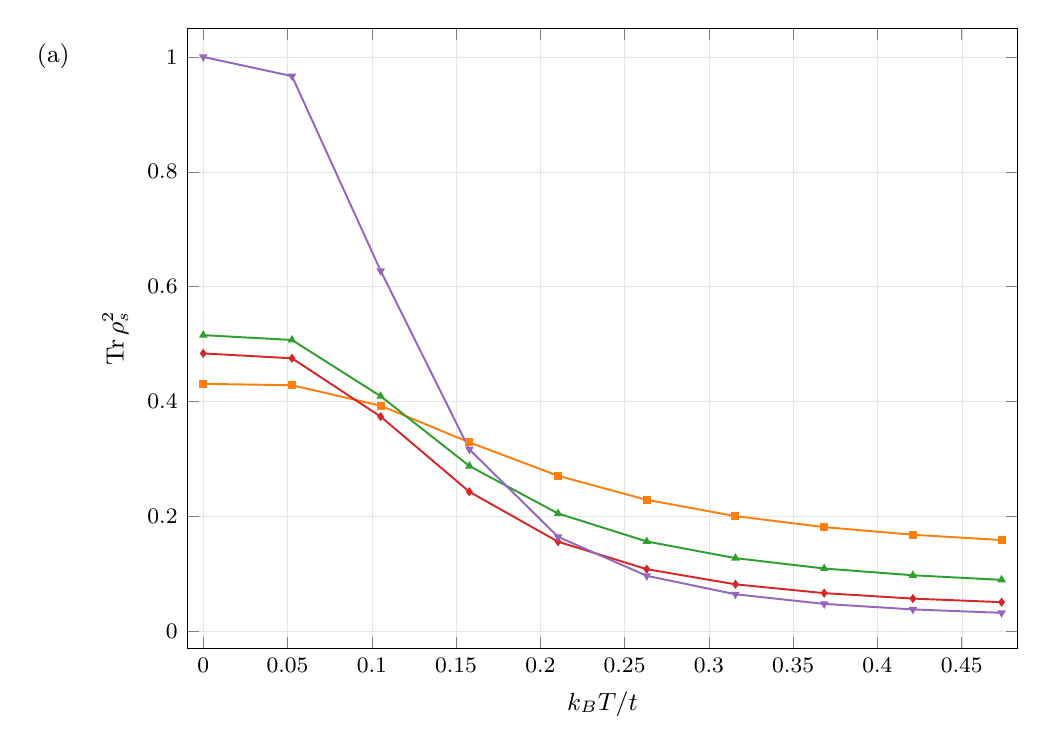
\begin{tikzpicture}
  \begin{axis}[
    width=\columnwidth,
    height=0.78\columnwidth,
    xlabel={$k_B T/t$},
    ylabel={$\mathrm{Tr}\,\rho_s^2$},
    grid=both,
    grid style={line width=.1pt, draw=gray!20},
    tick label style={font=\footnotesize\rmfamily, /pgf/number format/fixed},
    label style={font=\small\rmfamily},
    scaled ticks=false,
    legend style={font=\scriptsize\rmfamily, draw=gray!40, at={(0.5,1.03)}, anchor=south, /tikz/every even column/.append style={column sep=6pt}},
    legend cell align={left},
    legend columns=2,
    ymin=-0.03,
    ymax=1.05,
    xmin=-0.00947368,
    xmax=0.483158,
    after end axis/.append code={\node[anchor=east, font=\small\rmfamily] at (axis description cs:-0.13,0.954) {(a)};},
  ]
    \addplot[color=gmeC1, mark=square*, mark size=1.1pt, line width=0.7pt] coordinates {
        (0,0.430737) (0.052632,0.428267) (0.105263,0.392672) (0.157895,0.32884)
        (0.210526,0.270577) (0.263158,0.228688) (0.315789,0.200348) (0.368421,0.18118)
        (0.421053,0.167965) (0.473684,0.158625)
    };
    \addplot[color=gmeC2, mark=triangle*, mark size=1.1pt, line width=0.7pt] coordinates {
        (0,0.515511) (0.052632,0.507095) (0.105263,0.40914) (0.157895,0.287581)
        (0.210526,0.204949) (0.263158,0.156183) (0.315789,0.127174) (0.368421,0.109133)
        (0.421053,0.097368) (0.473684,0.089364)
    };
    \addplot[color=gmeC3, mark=diamond*, mark size=1.1pt, line width=0.7pt] coordinates {
        (0,0.483685) (0.052632,0.475235) (0.105263,0.373644) (0.157895,0.242758)
        (0.210526,0.155811) (0.263158,0.107936) (0.315789,0.081577) (0.368421,0.066237)
        (0.421053,0.056738) (0.473684,0.050523)
    };
    \addplot[color=gmeC4, mark=triangle*, mark size=1.1pt, mark options={rotate=180}, line width=0.7pt] coordinates {
        (0,1) (0.052632,0.96661) (0.105263,0.627503) (0.157895,0.316536)
        (0.210526,0.164201) (0.263158,0.096408) (0.315789,0.064274) (0.368421,0.047488)
        (0.421053,0.037884) (0.473684,0.031959)
    };
  \end{axis}
\end{tikzpicture}
